\section{Overview}\label{sec:overview}


Figure~\ref{fig:overview} shows the overview of our algorithm. 
The input 2D design layout of a carton consists of a set of cutting edges (solid lines) and folding edges (dashed lines).
%
Given the 2D layout, an undirected graph is built and a set of polygonal panels are extracted by finding the minimum cycles in the graph, as Figure~\ref{fig:overview}(b) shows. 
%Each face is filled with a unique color. %by ignoring the holes in the plane
The 2D layout therefore can be represented by a polymesh $\mathcal{L}=(V,E,P)$, where $V$ is the set of vertexes, $E$ is the set of all edges, and $P$ is the set of panels. 
The edge set $E=E_c\cup E_f$, where $E_c$ is the set of cutting edges, and $E_f$ is the set of folding edges.
%
To build a 3D carton model $\mathcal{M}=(V, E, P)$ from the 2D layout $\mathcal{L}$, while they share the same topology, we compute the 3D coordinates of all vertexes in $V$. 
%

However, it is not intuitive to analytically define the desired final 3D shape from a 2D layout. 
One possible way is detecting all the possible geometric constraints such as vertex merging, panel parallelism, orthogonality between adjacent panels, and then integrating all these possible constraints together to form a large equation system. 
But the challenge is that these local constraints can not well describe complicated and creative designs. 
Moreover, there are many ambiguities when detecting these constraints in a 2D layout that consists of many edges and panels in the same shape. 
%
Based on the observation that humans usually fold edges with a right angle to get a rough shape and then merge vertexes or edges to get a stable 3D carton, we propose a two-step algorithm. 
% Our algorithm consists of two steps. 
First, an initial 3D model (Figure~\ref{fig:overview}(c)) is constructed based on a specific angle along each folding edge, as described in Sec.~\ref{sec:initialization}.
The user can then manipulate and explore 3D shapes of the canton based on a series of suggestive operations provided by our system. 
%
The final model is shown in Figure~\ref{fig:overview}(e).
Details of each step will be introduced as following. 

% is finally built through the optimization based on the information acquired from user interaction. 
%\cxj{Modify this overview when you have new figure.}
%{\color{blue}{Furthermore, our system allows users modify the final 3D model to the desired shape, and automatically enforce the shape constraints reversely to the flat polymesh to get a deformable layout as shown in Figure~\ref{fig:overview} (f).}}

\begin{figure}
	\centering
	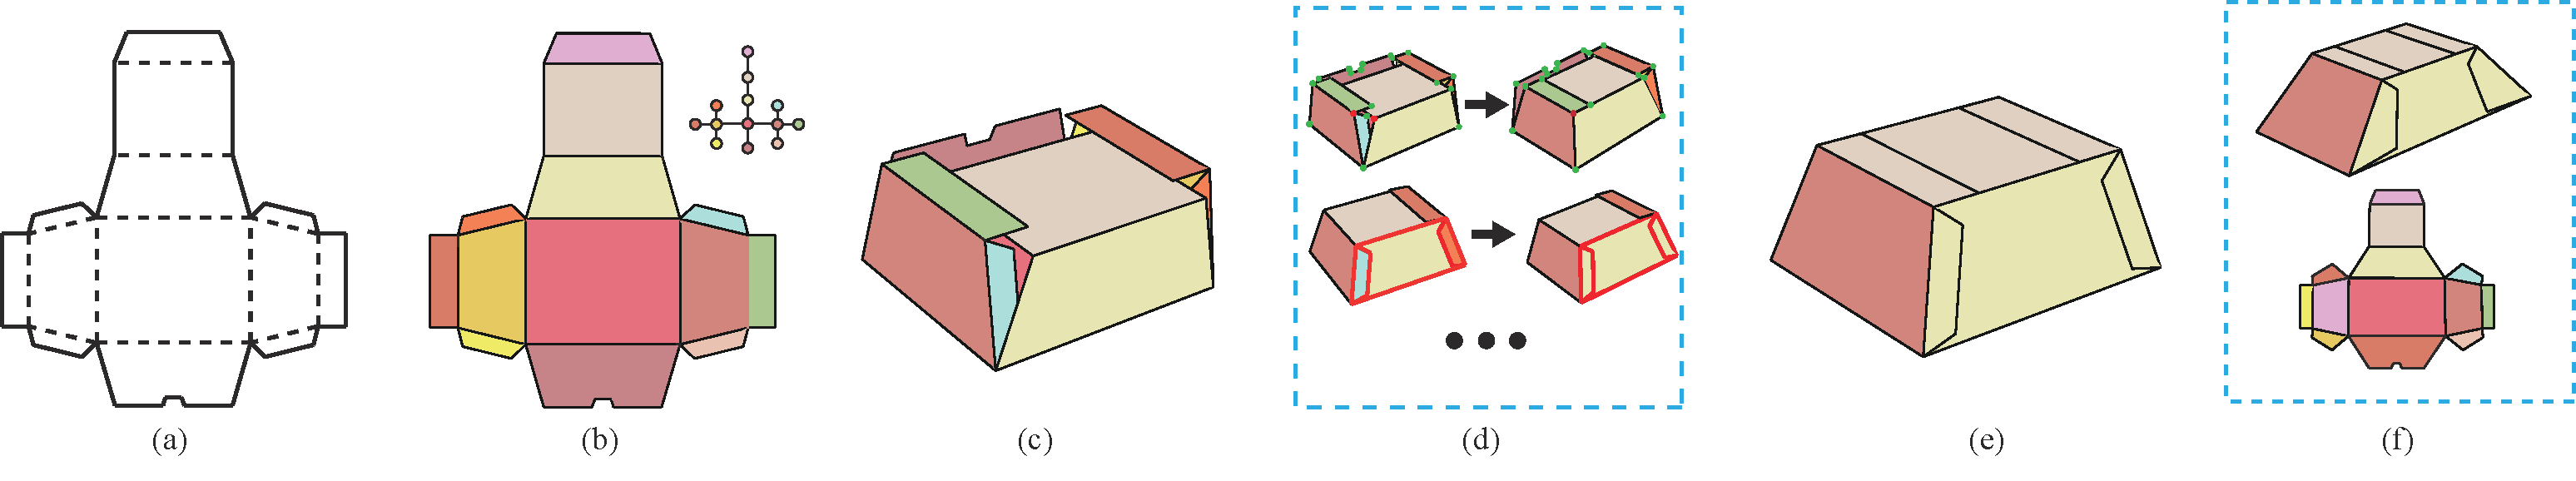
\includegraphics[width=0.9\textwidth]{images/overview}
	\caption{Given a 2D layout (a), we first extract its 2D mesh (b) with different panels in different color. By providing each folding edge with the same angle which is $\pi/2$, \xjmd{an initial 3D model can be constructed~(c). The final carton model (e) is built by a shape optimization technique based on a series of suggested geometrical constrains} (d).}
	\label{fig:overview}
\end{figure} 
 

